\providecommand{\main}{../../..}
\documentclass[\main/dresen_thesis.tex]{subfiles}
\renewcommand{\thisPath}{\main/chapters/appendix/additionalExperimentalTechniques}
\begin{document}

\chapter{Laboratory Instruments}
  \section{PPMS Evercool II - Vibrating Sample Magnetometry}
  \label{app:additionalExperimentalTechniques:vsm}
    \begin{figure}[ht]
      \centering
      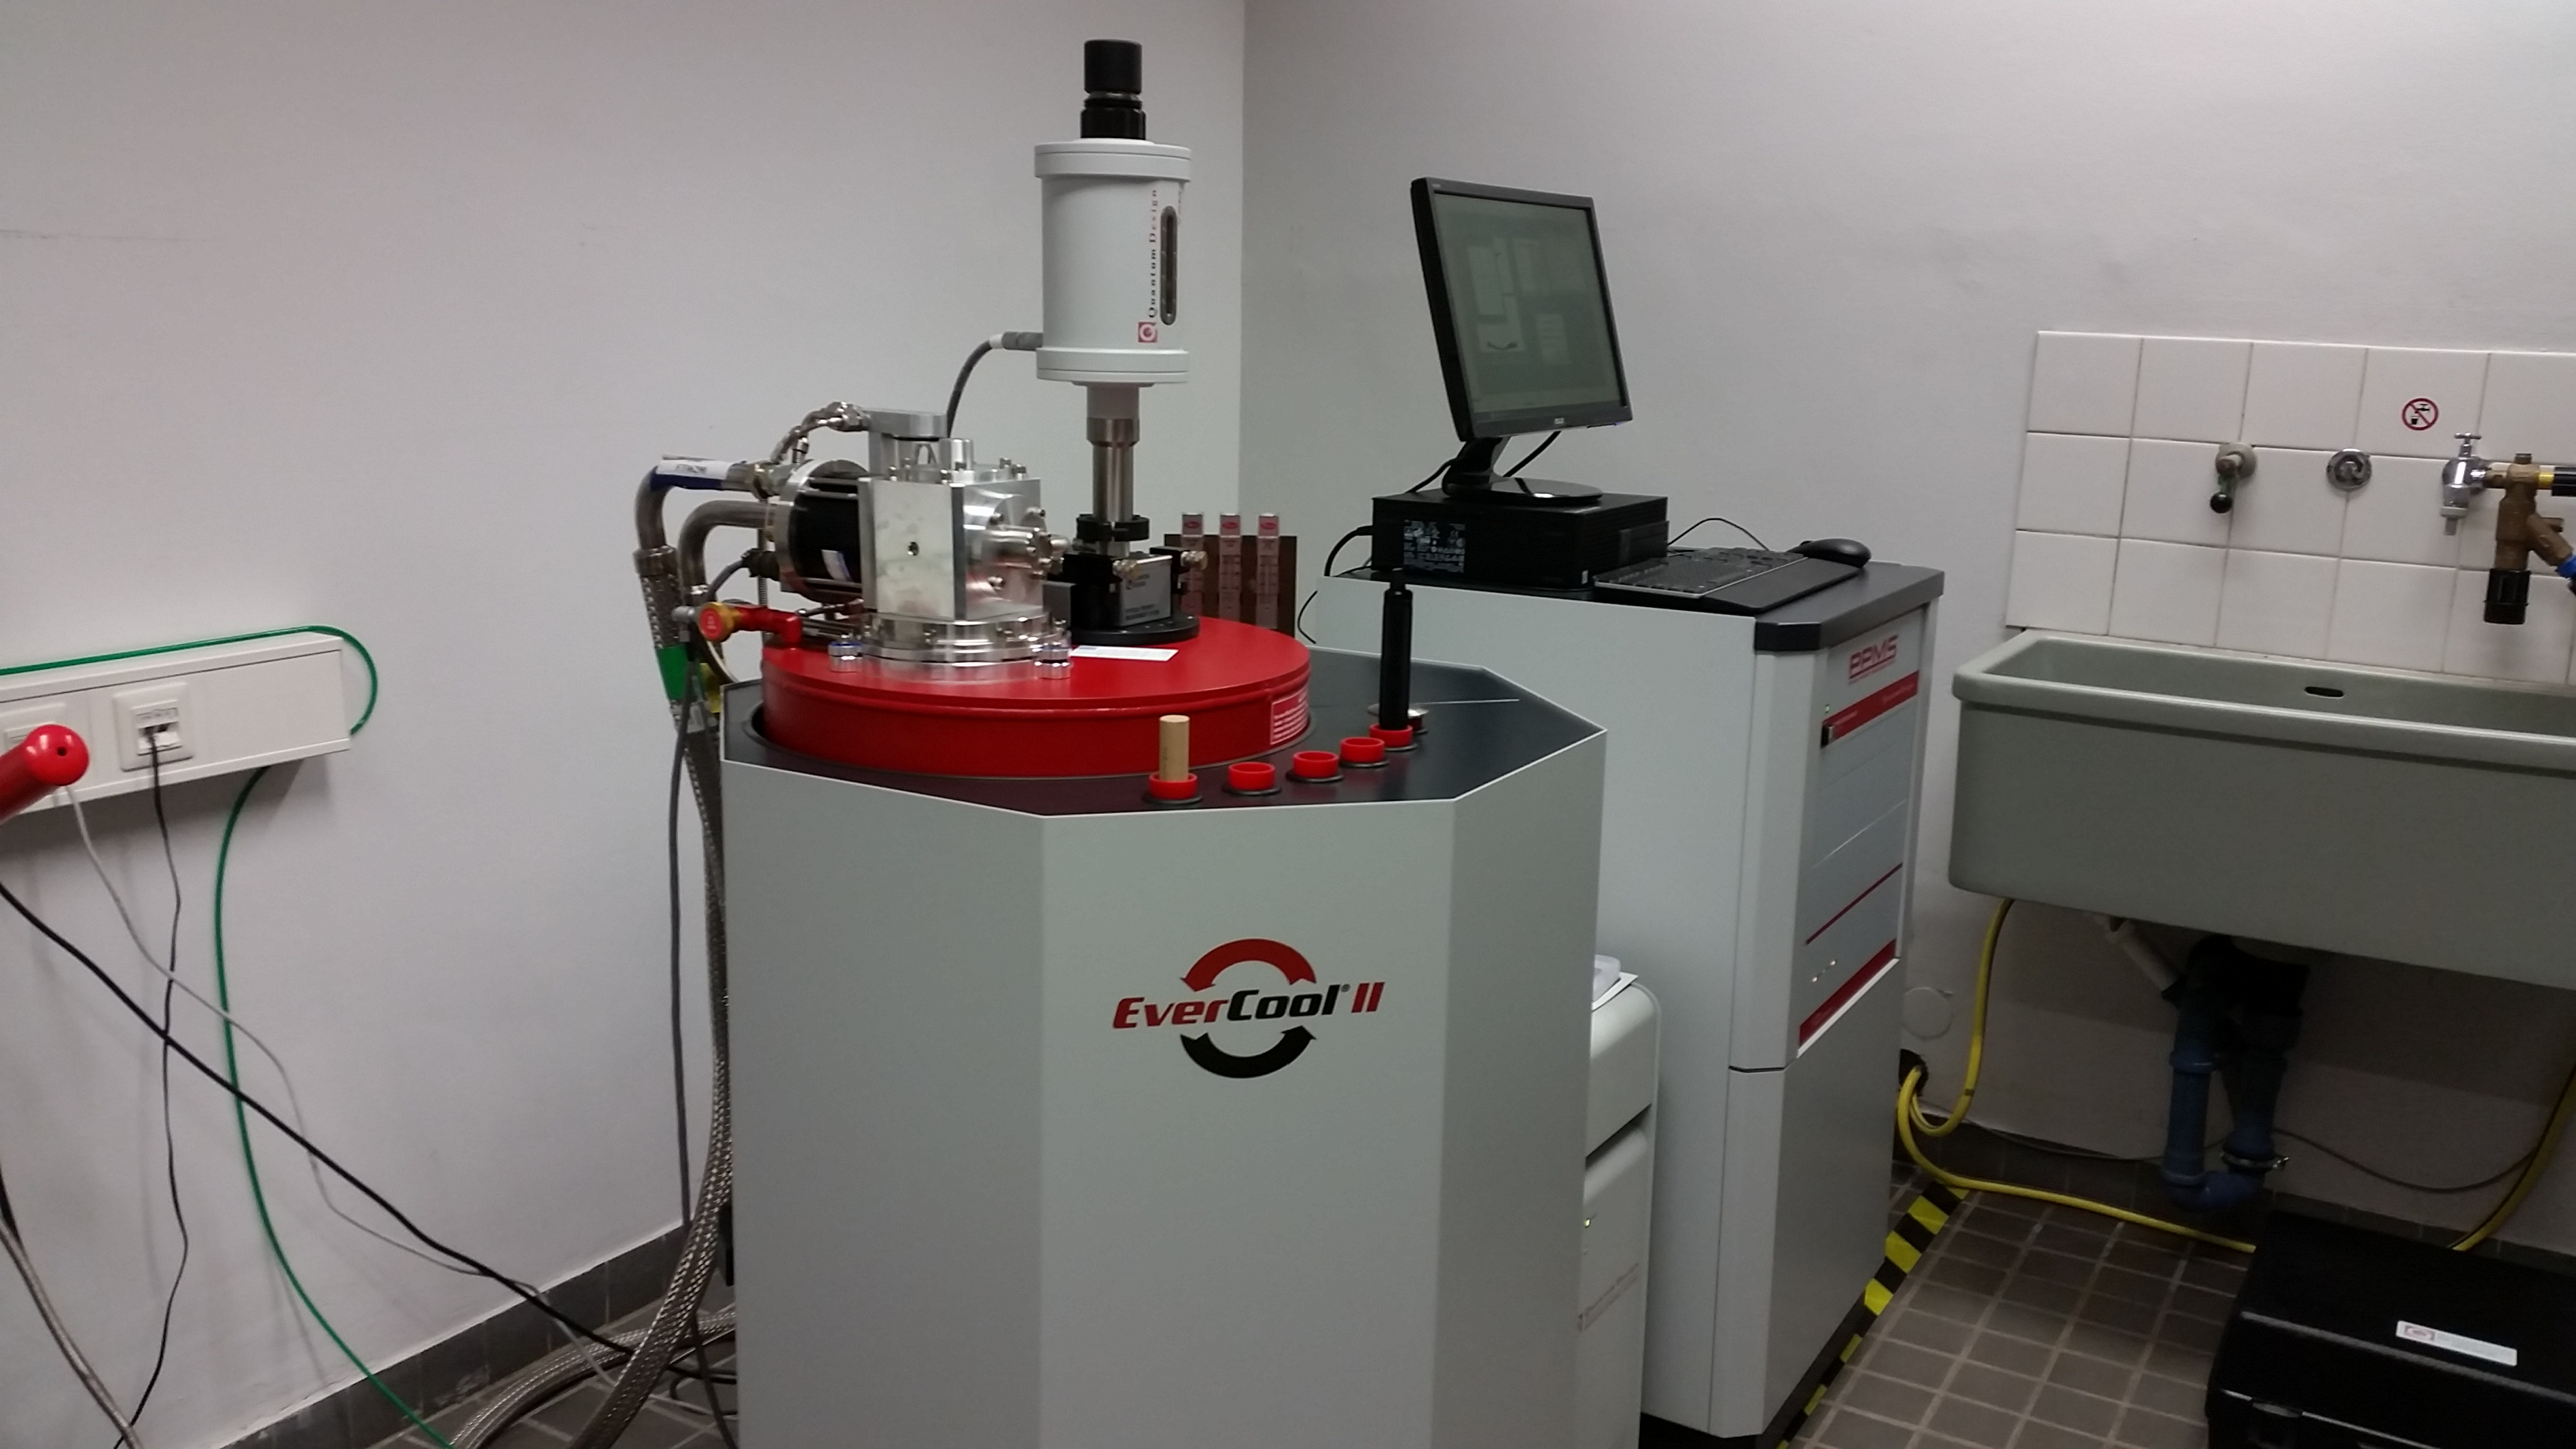
\includegraphics[width=0.7\textwidth]{instruments_ppms}
      \caption{\label{fig:appendix:instruments:ppms}The physical property measurement system (PPMS) Evercool II, which is used to measure the macroscopic magnetization properties by vibrating sample magnetometry.}
    \end{figure}
    During the course of this thesis a Evercool II from the company LOT Quantum Design was set up in the working group.
    The preparation of the laboratory for the instrument and support of the installation was performed in parallel to this thesis.

    The installed Evercool II has the option to choose between VSM (\refch{ch:methods:vsm}) and AC-Susceptometry, where the latter was not utilized in the scope of this thesis.
    A external field of up to $\pm 9 \unit{T}$ can be applied to magnetize samples, which are up to $5 \unit{mm}$ in diameter.
    Additionally the temperature can be freely varied in a temperature range of $2 \ldots 400 \unit{K}$.
    For this purpose, the Evercool II has a closed helium cycle.
    Meaning that only Helium lost during sample change or due to overpressure from fast temperature/field changes needs to be refilled.
    To cool the Helium compressor of the helium cycle, a water-cooling solution has been installed.

    The VSM option has a noise level in the order of $0.1 \ldots 1 \unit{\musf emu}$, depending on the temperature and external field.

  \section{Bruker D8 Advanced - X-Ray Reflectometry}
  \label{app:additionalExperimentalTechniques:xrr}
  \begin{figure}[ht]
    \centering
    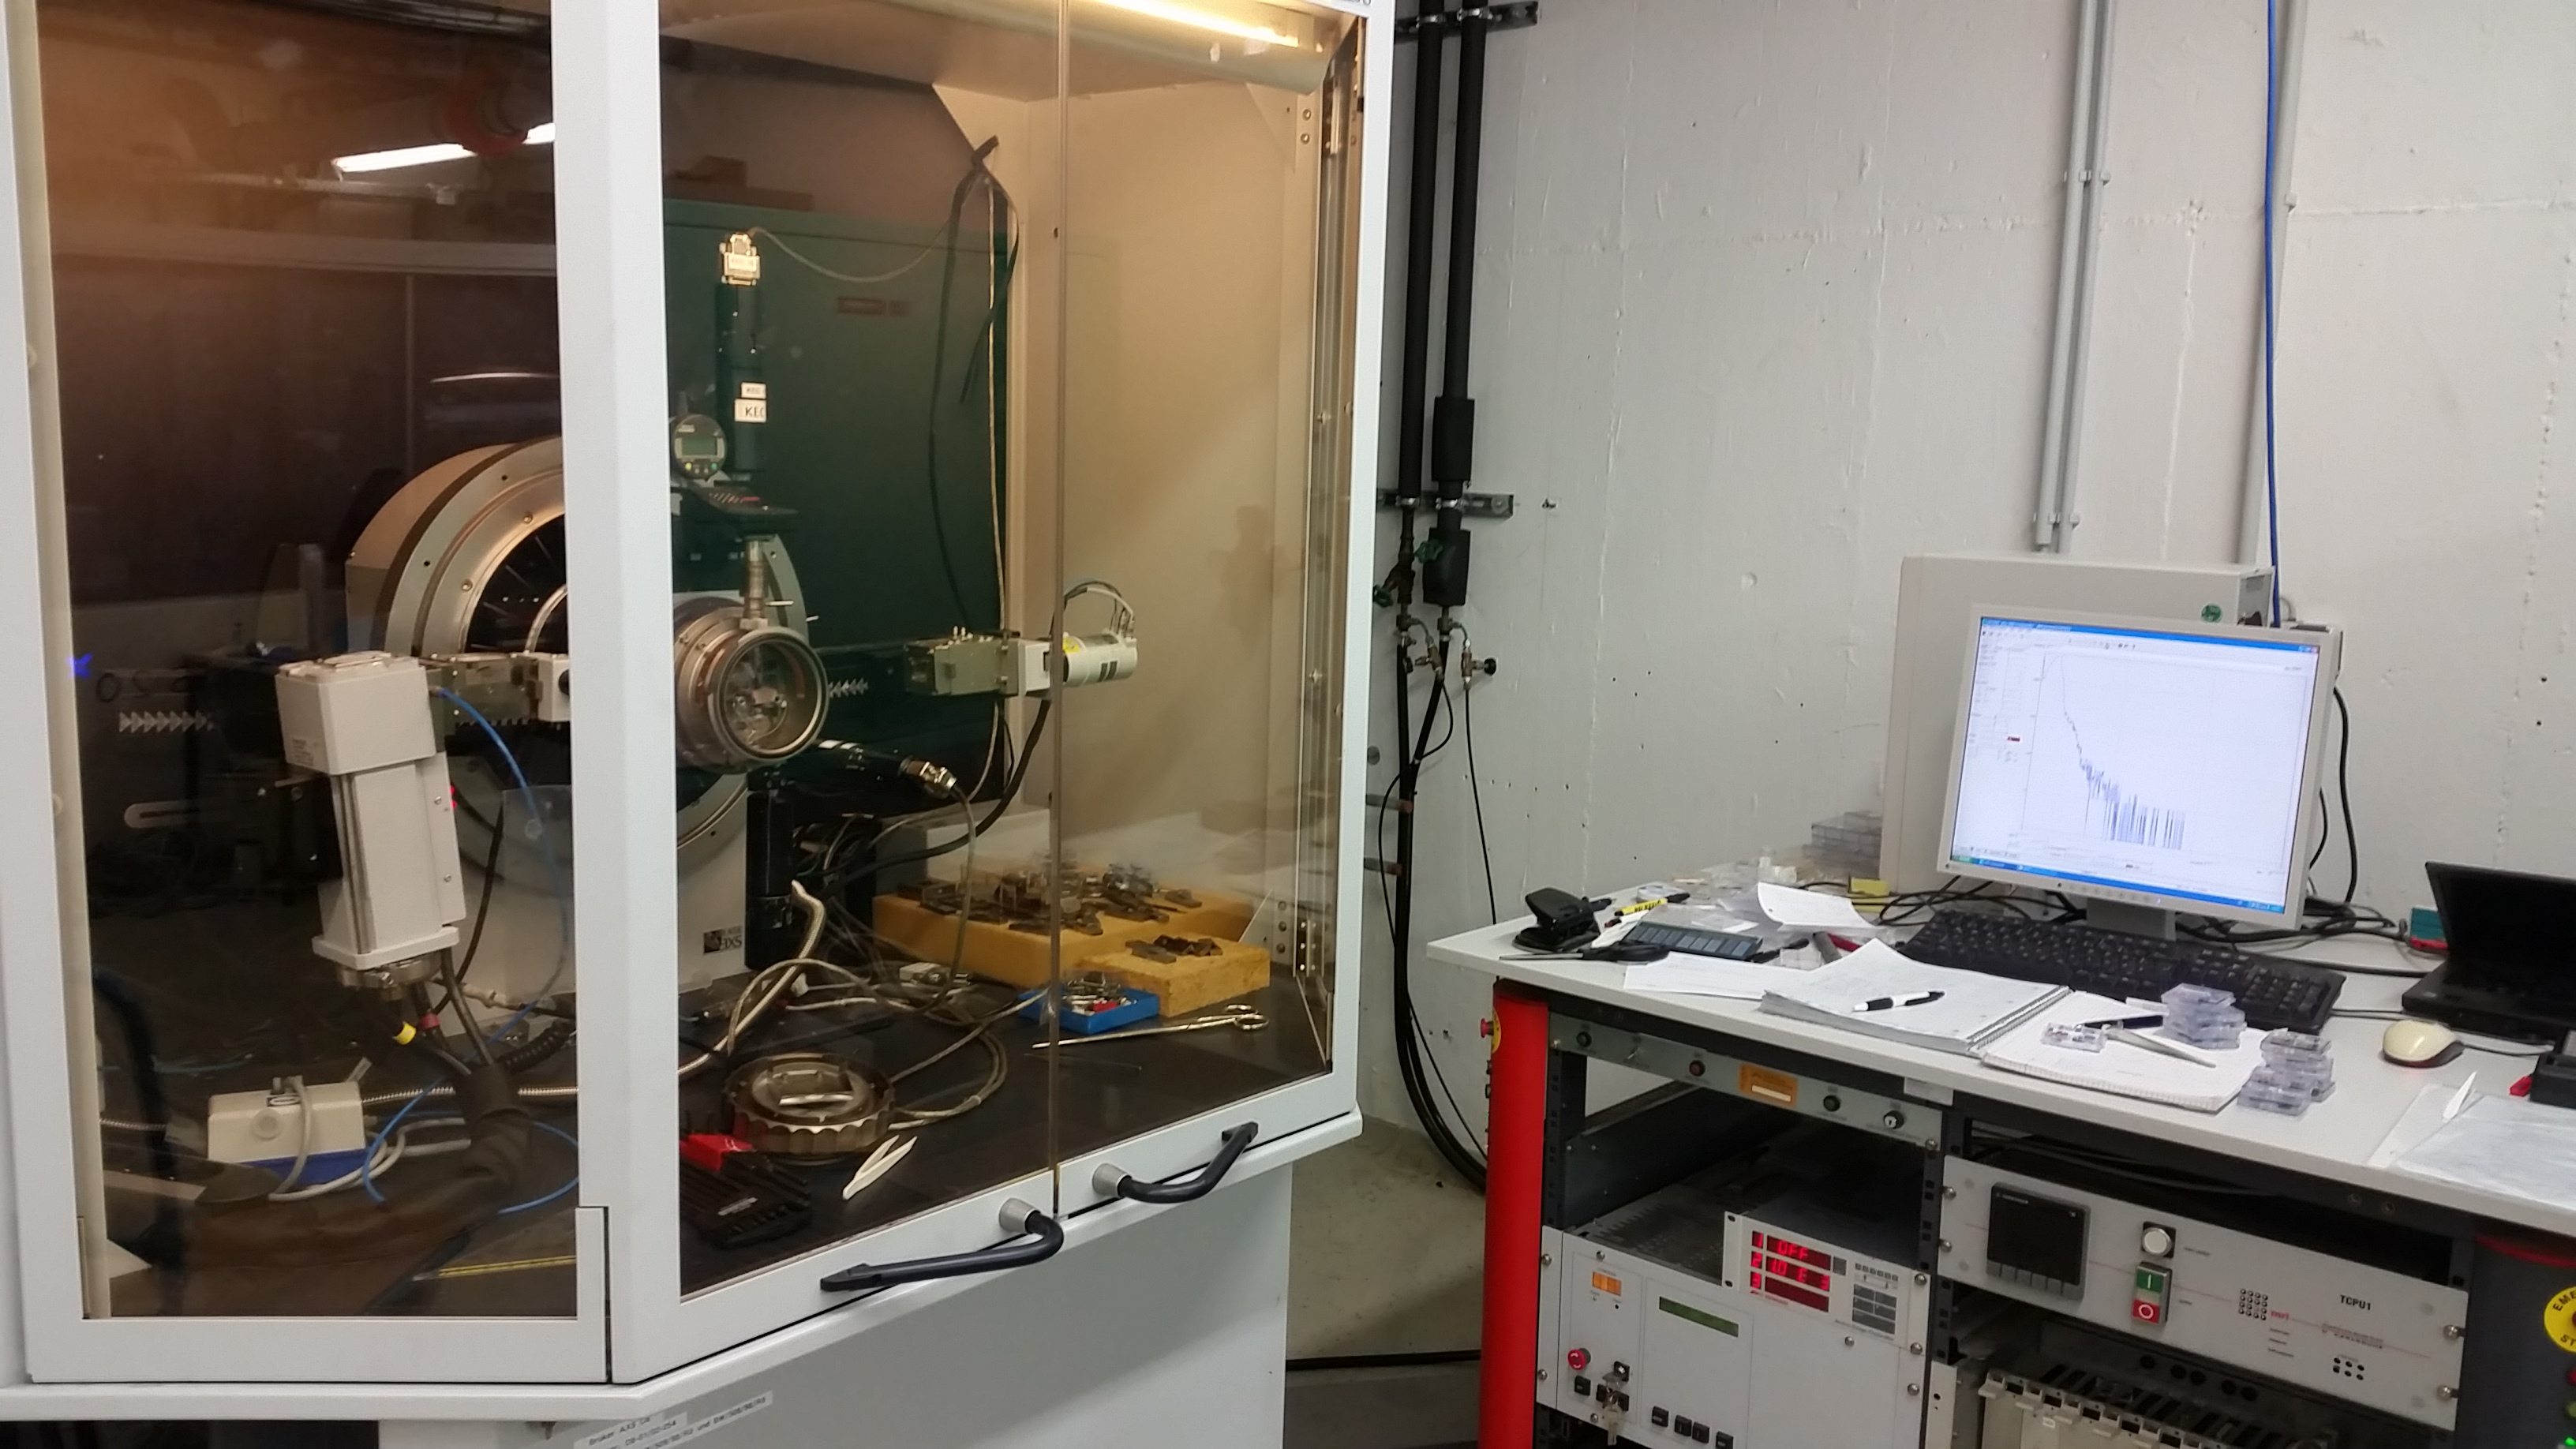
\includegraphics[width=0.7\textwidth]{instruments_brukerD8}
    \caption{\label{fig:appendix:instruments:brukerD8}Bruker D8 instrument, which can be used for X-ray reflectometry and X-ray diffraction.}
  \end{figure}
  To perform XRR experiments, described in \refch{ch:methods:xrr}, the Bruker D8 instrument in the \textsc{Forchungszentrum J\"ulich} was used.
  The Bruker D8 operates with a Cu-K$\alpha$ source and has two Goebel mirrors installed to direct the beam in front and after the sample.
  The source and the detector are both installed at a fixed distance of approximately $30 \unit{cm}$ from the sample position and can only moved on a circle.
  At the source and detector, slits of $0.2 \unit{mm}$ width are installed.
  Additionally, absorber materials can be placed in the beam path electronically, in case the the photon count on the detector is larger than the electronics can handle, \eg when the direct beam is measured.

  \begin{figure}[ht]
    \centering
    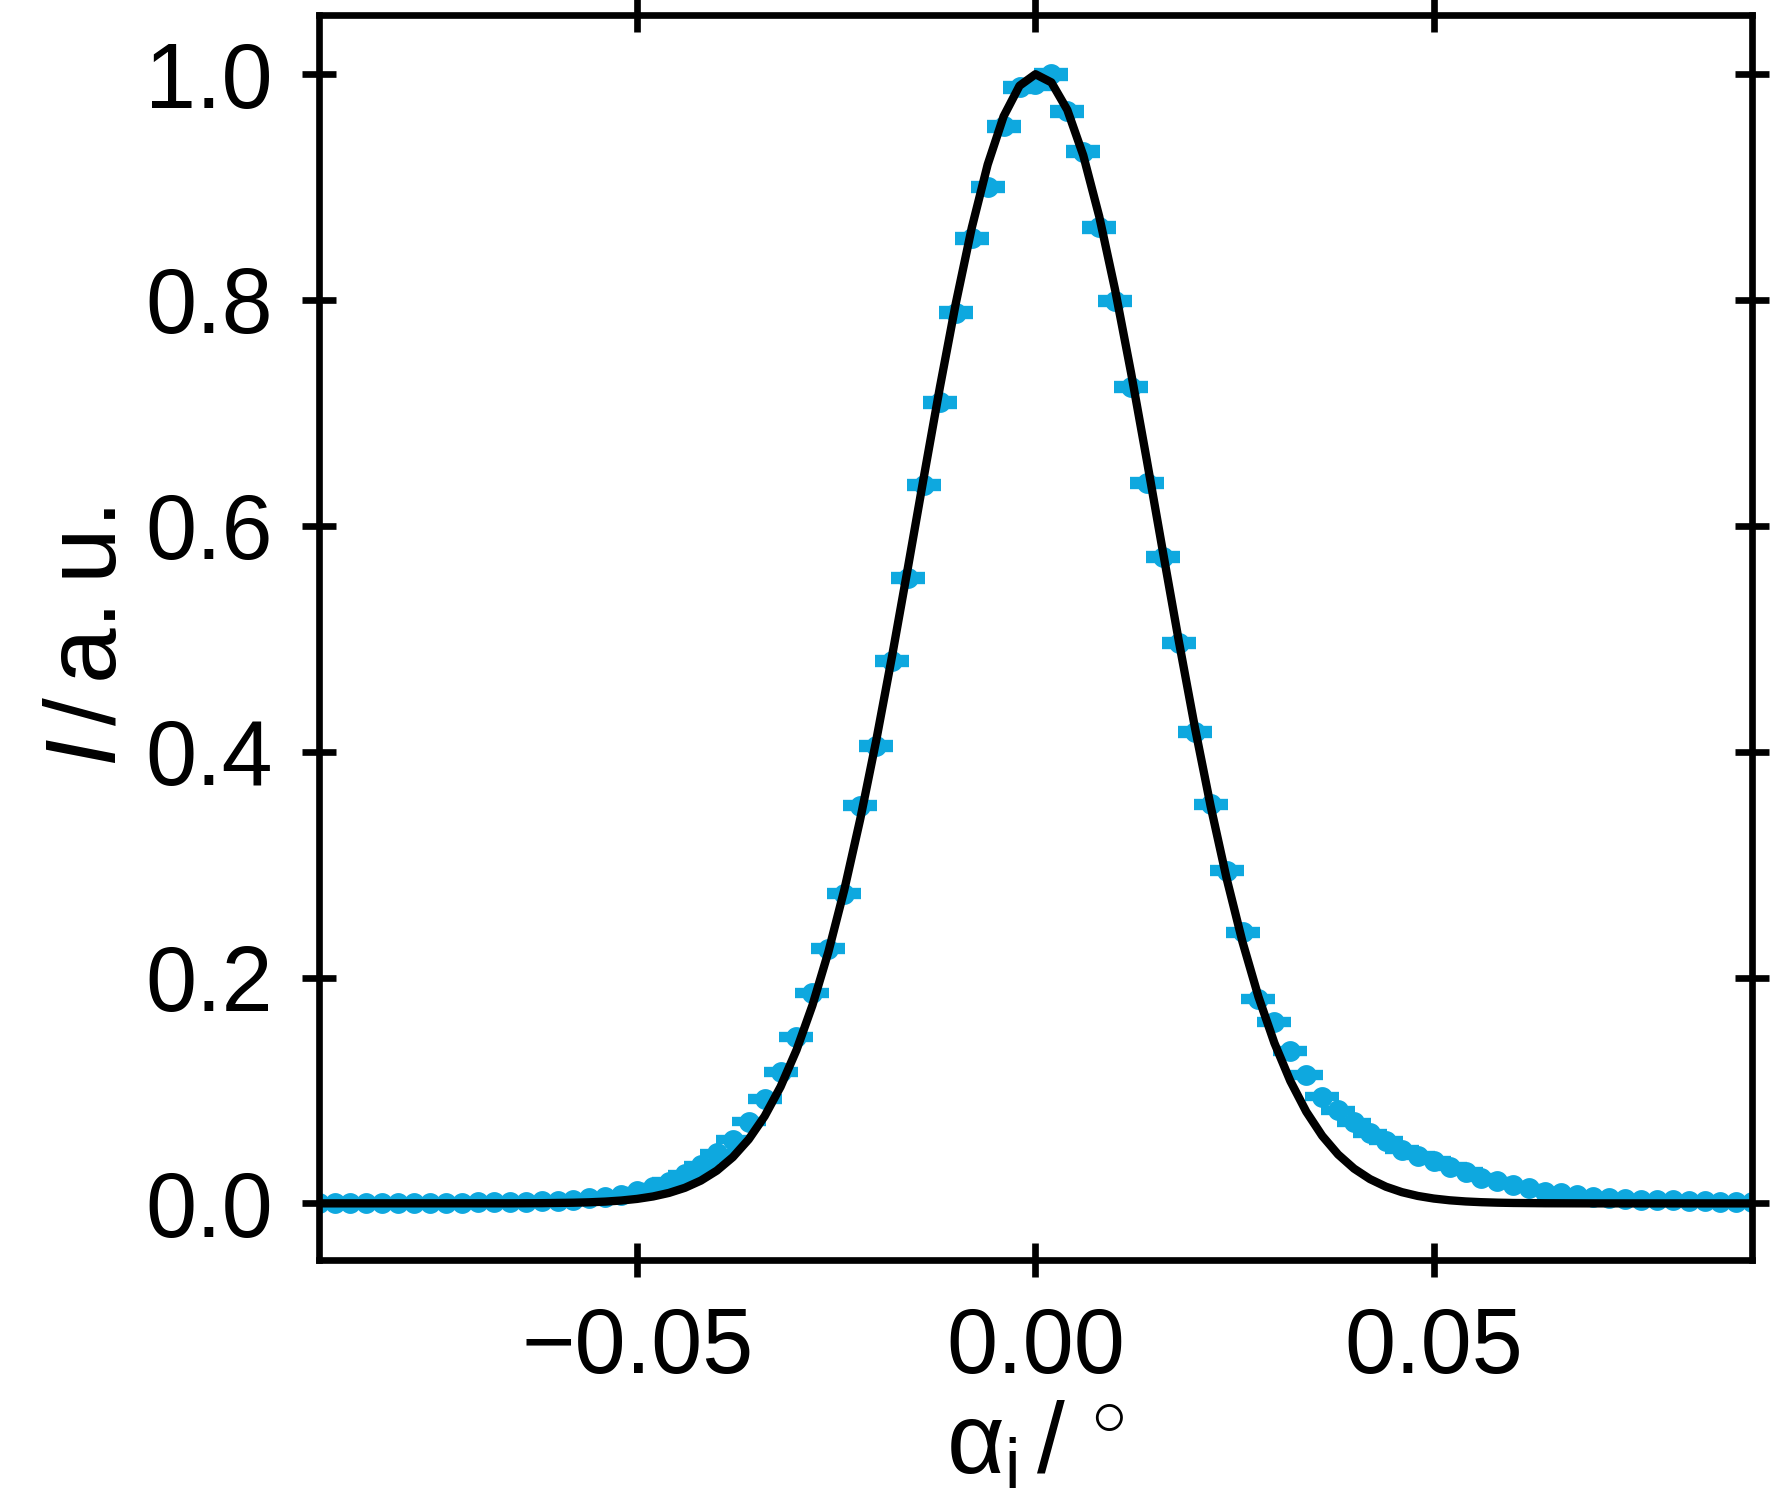
\includegraphics{appendix_instruments_brukerD8DirectBeam}
    \caption{\label{fig:appendix:instruments:brukerD8DirectBeam}Direct beam scan of the Bruker D8 instrument at a beam slit size of $0.2 \unit{mm}$, modelled by a gaussian function to estimate the divergence.}
  \end{figure}

  By scanning the direct beam of the instrument, when no sample is placed in the beam path, the angular divergence is estimated as shown in \reffig{fig:appendix:instruments:brukerD8DirectBeam}.
  The best fit with a gaussian function results in a divergence of $\Delta \alpha_i \eq 0.01510(4) ^\circ \eq 2.635(7) \cdot 10^{-4}.$, which corresponds for the distance of $30 \unit{cm}$ to a width of $0.15 \unit{mm}$, which coincides well with the slit size.


  \section{X-Ray Diffraction}
  \label{app:additionalExperimentalTechniques:xrd}
  The presented XRD profiles in this thesis were measured in collaboration with the group of Daniel Nižňanský from the Department of Inorganic Chemistry at the Charles University in Prague.
  They use 

  \section{Neon Zeiss 40 - Scanning Electron Microscopy}
  \label{app:additionalExperimentalTechniques:sem}
  \begin{figure}[ht]
    \centering
    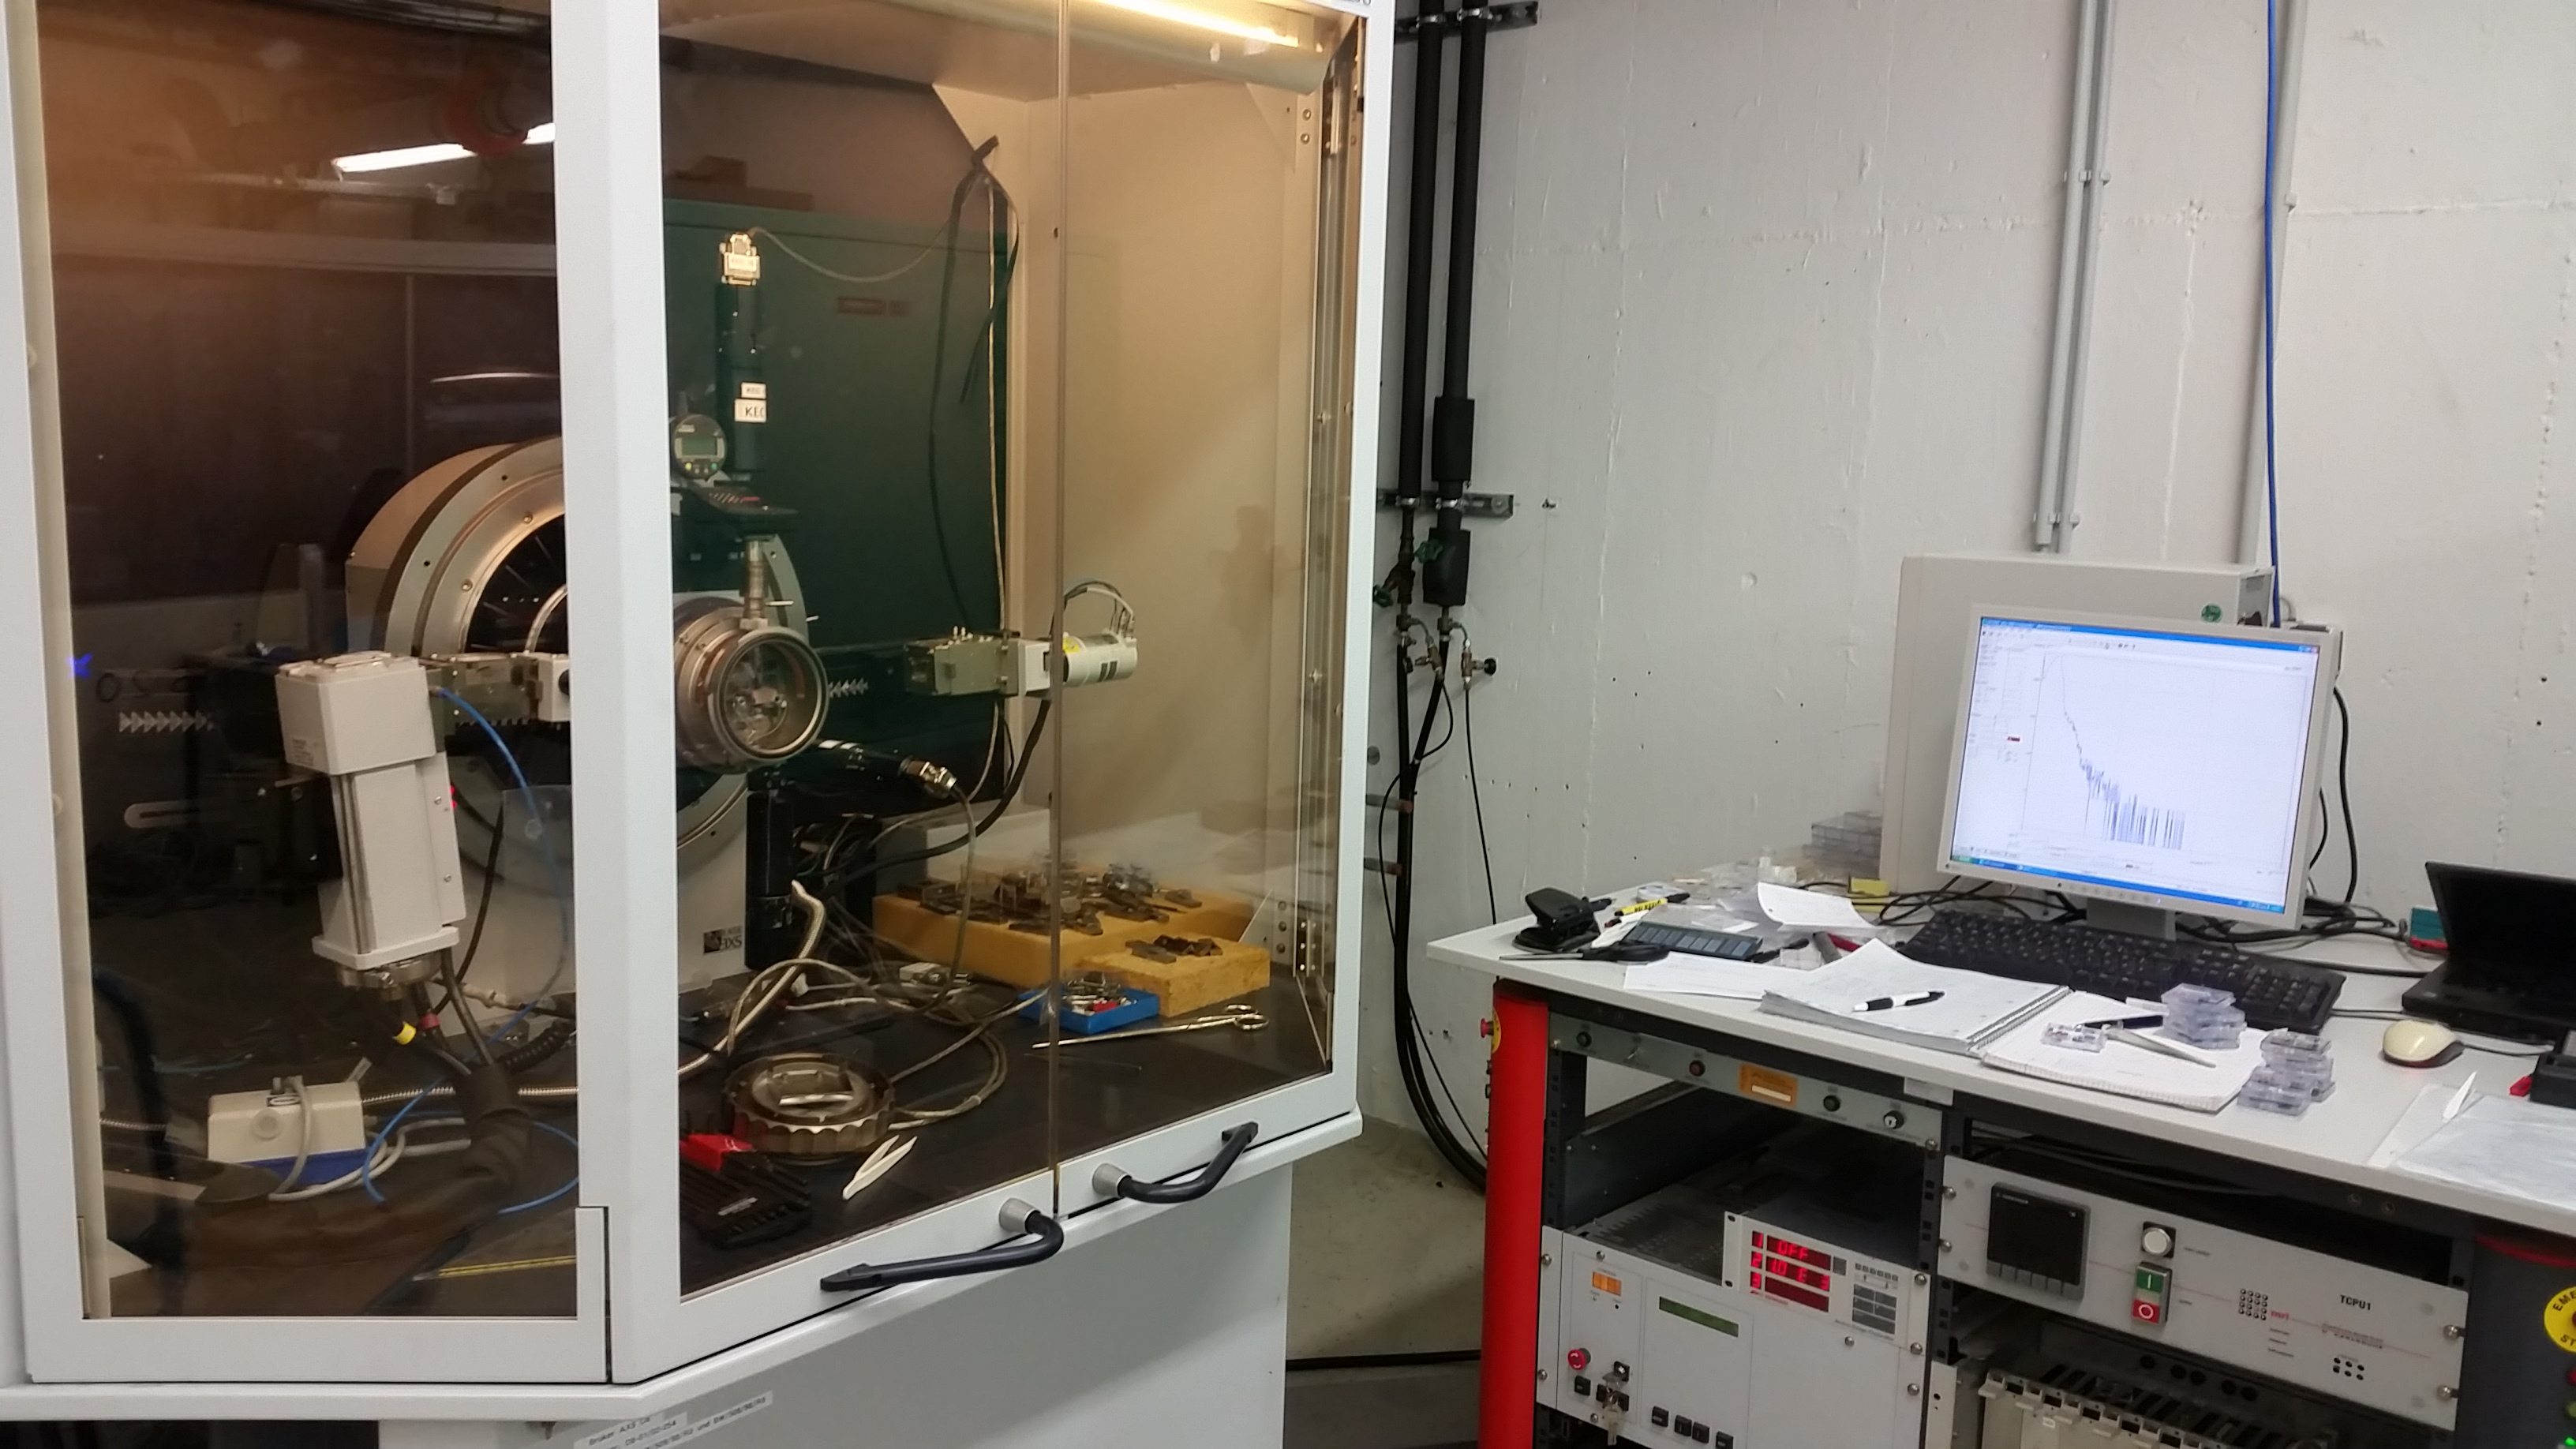
\includegraphics[width=0.7\textwidth]{instruments_brukerD8}
    \caption{\label{fig:appendix:instruments:SEM}Bruker D8 instrument which can be used for X-ray reflectometry and X-ray diffraction.}
  \end{figure}

\end{document}
